\chapter{Design}

\section{Outline}
Given that we want to be able to generate tests based on requirements require structure and a touch of semantics. For the latter, we need to infer some minimal understanding into the test generation system of what the different components are (actor, action, \dots). For the structure part, we must enforce some sort of categorization such as defining the level, scope and composition of a use case. By composition is meant the different parts; scenario, pre- and post-conditions.\\
This structure and semantics are best defined by the stakeholder that knowns the problem domain by heart; the customer of the software. There are however some challenges in extracting the domain knowledge from these stakeholders which is discussed in the next section.

\section{Stakeholders}
The problem in attaining broad coverage of use cases, and therefore completeness in requirements i primarily that, from the customer perspective, that they feel very overly-verbose and usually too formal in nature. For software engineers, the opposite is usually the case. They feel that the use case descriptions are not structured nor elaborate enough for use in, for instance, code stub generation.

More structure, however, could be helped along the way with proper tooling. Hiding some of the complexity of the constrains of a data model behind a simple user interface supplying dragable components and providing immediate visual feedback in the form of textual use case representation (or a diagram) could "cheat" the customer into adding the needed structure to the use case model.

What is in the customers interest is having acceptance tests match the use cases as closely as possible. Preferably, the should be able to be automated as well. Figure \ref{fig:use_case_creation_activity_diagram} shows an activity diagram involving three actors, the customer, the engineer and the system\footnote{Use case system}. In this diagram, the customer authors use cases while adding missing definitions not already in the tool. A definition is textual description of a concept which may be -- for instance -- an actor, role or action. This description is then given a unique name, that may correspond to a concept already found in the domain model. The domain model, if defined beforehand, could also be thought to be a part of the built-in declarations.
\subsection{Developer}
% What is to be gained for this stakeholder?
There are different levels to write the use-case tests on;
%\begin{description}
%  \item [Manually:] all the tests and the domain model and logic
%  \item [Partially automatic:] either by writing up support code for the domain model manually, and generates the use cases, or the other way around.
%  \item [Fully:] automatic.
%\end{description}


%\section{Brainstorm}
%\section{Costumer overview}
The problem in attaining broad coverage of use cases, and therefore completeness in requirements i primarily that, from the customer perspective, that they feel very overly-verbose and usually too formal in nature. For software engineers, the opposite is usually the case. They feel that the use case descriptions are not structured nor elaborate enough for use in, for instance, code stub generation.

More structure, however, could be helped along the way with proper tooling. Hiding some of the complexity of the constrains of a data model behind a simple user interface supplying dragable components and providing immediate visual feedback in the form of textual use case representation (or a diagram) could "cheat" the customer into adding the needed structure to the use case model.

\begin{figure}[h]
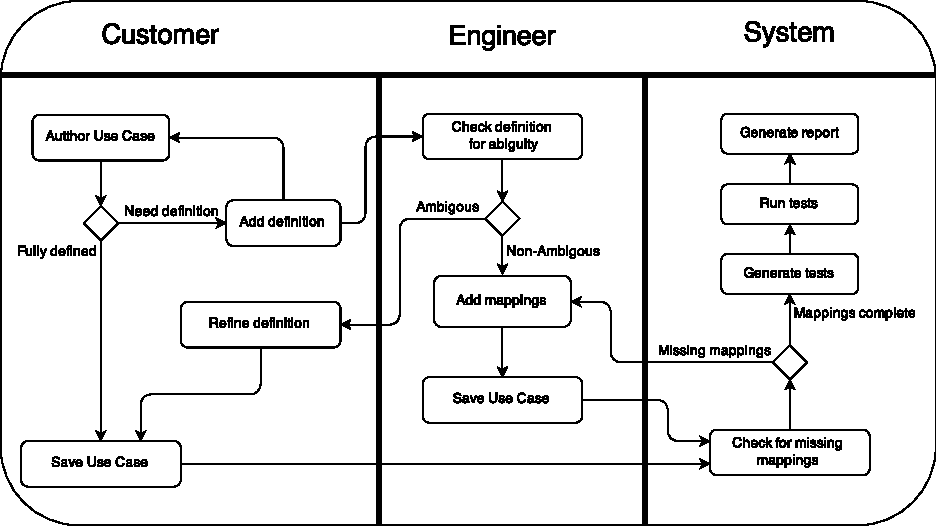
\includegraphics[scale=0.75]{img/use_case_creation_activity_diagram}
\centering
\caption{Use case creation with different actors}
\label{fig:use_case_creation_activity_diagram}
\end{figure}

What is in the customers interest is having acceptance tests match the use cases as closely as possible. Preferably, the should be able to be automated as well. Figure \ref{fig:use_case_creation_activity_diagram} shows an activity diagram involving three actors, the customer, the engineer and the system\footnote{Use case system}. In this diagram, the customer authors use cases while adding missing definitions not already in the tool. A definition is textual description of a concept which may be -- for instance -- an actor, role or action. This description is then given a unique name, that may correspond to a concept already found in the domain model. The domain model, if defined beforehand, could also be thought to be a part of the built-in declarations.

\begin{figure}[h]
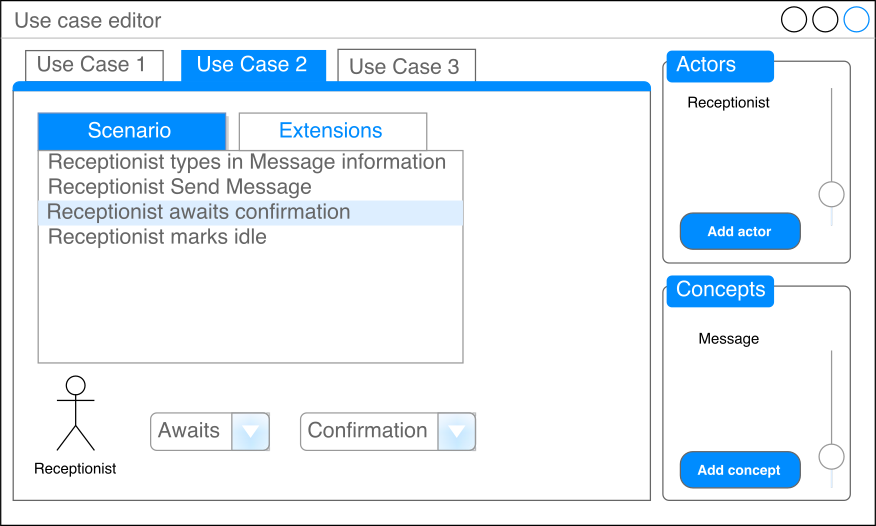
\includegraphics[scale=0.9]{img/test_case_ui}
\centering
\caption{Use case editor UI mockup}
\label{fig:use_case_editor_mockup}
\end{figure}

Whenever there is a new use case, a change to an existing use case, or simply a definition, the system should try to generate tests from the new information. If this step fails it is likely due to insufficient concept mappings. From here, a software engineer must manually map individual definitions to system macro-functionality or, possibly the use case could be linked to an existing manually written test, if the generation step is not possible for some reason. A mockup of a user interface from the customer point of view is shown in figure \ref{fig:use_case_editor_mockup}. A list of available actors (only containing one element, however) is shown on the right hand side. The main part of the window contains the use case currently being worked on. The bottom part of the window is the edit part, where dropdown lists of actions and targets resides.


\section{Proposed solution}
"Side-cart" tool that (maybe) uses natural language processing. The developement is supported by a two-sided approach. Both top-down and bottom-up. Meaning that design an implementation will go hand-in-hand and hopefully lead to a good middle-road.
%TODO something about existing approaches.
%TODO Step-wise go through the enhancement process.
%  - Basically, autogenerate the use case action code line
%  - Infer some Class dependencies, which then becomes Framework dependencies.
%Definition dictionary
% Remember that an actor has a set of goals, which he/she wants to realize through the system. Actor can be  primary (typically people) or supporting (provides service or information) - passive.
% A good goal has a verb/noun combination.
%REMEMBER TO TAKE INTO ACCOUNT <INCLUDE> use cases -- Basically extensions
This section takes starts from a use case description, and tries to go through the steps needed to convert it into an acceptance tests. The use case used in this text is simplified and outlined in verbatim text seen in listing \ref{lst:uc-simple-example}.\todo[inline]{Check context, and make sure it leads in to this.}.
\begin{lstlisting}[frame=single,style=usecase, caption=Use case example, label=lst:uc-simple-example]
Scenario:
  Receptionist types in message
  Receptionist sends message
  Receptionist marks state as ready 
Preconditions:
  The receptionist is created
  The receptionist is logged in
Postconditions:
  The message is stored
  The receptionist is ready to handle the next call
\end{lstlisting} 
Translating this example, we first identify the domain concept contained within the statements in the text. In this case, we here observe that it includes the concept ``message'' a ``receptionist'' actor. additionally; some interaction between the message and the actor, which we define as actions.\\
In listing \ref{lst:uc-simple-example-highlighted} we have highlighted the different parts of the use case, using an orange color for actors, green for actions, blue for domain concepts, and a dark red for attributes. Using this highlight, it illustrates the abstract interpretation and the interaction between the different part very well. It also reveals very clearly which archetype (actor, concept \dots) each of the different parts should have. 
\todo[inline]{More elaborate text here}.
\begin{lstlisting}[frame=single,style=usecase, caption=Use case example with its different parts highlighted, label=lst:uc-simple-example-highlighted]
Scenario:
  @\color{orange} Receptionist@ @\color{dkgreen}{types in}@ @\color{blue}{message}@
  @\color{orange} Receptionist@ @\color{dkgreen}{sends}@ @\color{blue}message@
  @\color{orange} Receptionist@ @\color{dkgreen}{marks state}@ as @\color{blue}{ready}@
Preconditions:
  The @\color{orange}receptionist@ is @\color{dkred}logged in@
Postconditions:
  The @\color{blue}message@ @\color{dkred}is stored@
  The @\color{orange}receptionist@ @\color{dkred}is ready@ to handle the next call
\end{lstlisting} 
Based upon the information in listing \ref{lst:uc-simple-example-highlighted}, we could create an abstract interpretation that generates a test that looks like listing \ref{lst:uc2_example_test_code}.
Each of the concepts in this example is mapped to a class, that could likely be stubbed out automatically by the test tool.\\\\
Given the amount of information in (and markup of) the use cases, we can easily generate code such as the one shown in listing \ref{lst:uc2_example_test_code}. But these functions are still very high-level, and doesn't assert anything about the system being tested. To do this, we need to fill in the methods used on our receptionist and message object.
\begin{lstlisting}[caption=Suggestion of generated test case,label={lst:uc2_example_test_code}]
boolean test (receptionist, message) {
  // Scenario
  receptionist.types_in (message);
  receptionist.sends (message);
  receptionist.marks_state (idle);
  
  // Postcondition
  return
    message.is_stored() AND
    receptionist.is_ready();
}
\end{lstlisting}
Going through the test case, from the top, we can see that the \texttt{receptionist.types\_in~(message)} method operates on the receptionist actor call, and requires knowledge of the ``message'' domain concept. Furthermore, we known from the domain analysis that \emph{is not part} of the use case, that the action of typing in a message is actually a creation of message. So, before being able to test it, we need some way of simulating the message creation and -- more concretely -- fill in the actual message content. Conceptually, this is some sort of content generator. A concrete implementation could be a simply ``dummy object'' or an object that is initialized with random content. Once the message object is mapped to a content generation function, we will be able to fully generate the test. The content generation function would probably still need to be hand coded, as this is example data.\\\\
The next statement; \texttt{receptionist.sends (message)} can be classified as a store function. It takes the argument ``message'' and makes it available for other actors to access later on, by storing it persistently. This is typically done using a database or file store. By mapping a message to a message store, we can remap an ``enqueue'' method of the message object, which needs to have a notion of where it is, or should be stored. This is realized by having a ``messageStore'' interface which is a service interface object that, can actually be originating directly from the code base of the system under test.\\\\
The final statement in the scenario is \texttt{receptionist.returns\_to (ready\_state)}. This is actually a mutation function that alters the state of the receptionist actor. This state change could be global and should then  be updated multiple places, which then leads to additional ``state-store'' dependencies. Here, we also note that there is a concept of a ready\_state this is an explicit state change that could, possibly be linked to a state machine contained within the receptionist actor object.\\\\
The final thing done in the tests, is the postconditions. In this case, we treat the postcondition as a boolean attribute of the concept which it refers to. The general assumption is that pre- and postconditions are expressions that must always be true, and must refer to a concept previously referred to in the scenario. So for the \texttt{receptionist.is\_ready()} predicate we can map it to the internal state of the receptionist being equal to the ``ready'' state.\\\\
The mapping can be described in a textual language such as shown in listing \ref{lst:mapping_language_concept} where we initially state the domain concept name -- which is in this case Receptionist -- and the requirements, properties and mappings it has, plus which functionality it provides. The requirements are which other domain concepts are needed by this one. The properties are the boolean properties that are used in predicates and the ``provides'' section are functions that are either used as internal auxiliary functions, or exported functions that other concepts may use.
%Prior to running the tests, the two objects ``message'' and ``receptionist'' needs to be initialized.
%The question is then how much more needs to be added. Can we use some stereotyping to increase the semantics of the annotated use cases? Such as 'storage' for message, and 'actor' for receptionist.
%So last question; who does what, and how much can be automated?
%The first part of the job; typing in the use cases is a manual process that should be done in close cooperation with -- and preferably by -- the stakeholder involved in the use case. So a use case involving an accountant actor should be typed by a accountant representative expected to be using the system, once finished.

\begin{lstlisting}[caption=example language for mapping concepts,label={lst:mapping_language_concept}]:
Receptionist:
  requires:
    MessageContentGenerator messageContentGenerator
    ReceptionistState currentState = ReceptionistState.Unknown
  
  provides:
    changeState (ReceptionistState rs) -> currentState = rs
  
  maps:
    sends_message (Message msg) -> msg.enqueue()
    types_in (Message msg) -> msg.content = messageContentGenerator.next().content
    returns_to (ReceptionistState newState) -> this.changeState (newState)

  properties:
    is_ready -> receptionistState == ready
\end{lstlisting}
The mappings are, in this conceptual model, alias functions to ``real methods'' already provided in the code base of the software under tests, or to functions of other domain concepts. This is probably not feasible in praxis, and will probably be a programing code template instead.

\begin{lstlisting}[caption=Pseudo code representing Receptionist domain actor,label={lst:code_for_receptionist_domain_actor}]
class Receptionist {
   MessageContentGenerator messageContentGenerator= ...;
   ReceptionistState receptionistState = ...;
  
  void types_in (message) {
  	message.updateContent(messageContentGenerator.content);
  }
  
  void sends (Message message) {
    message.enqueue();
  }
  
  // Alias function.
  void returns_to (State newState) {
  	changeState (newState);
  }
  
  void changeState (State newState){
  	receptionistState = newState;
  }
  
  boolean is_ready() {
    return receptionistState == ready;
  }
}
\end{lstlisting}

\begin{lstlisting}[caption=Pseudo code representing Message domain concept,label={lst:code_for_domain_concept}]
class Message {
  RESTMessageClient messageStore = ...;
  
  void enqueue() {
    messageStore.enqueue(message);
  }

  boolean message.is_stored() {
    messageStore.contains(this);
  }
}
\end{lstlisting}

\begin{figure}
 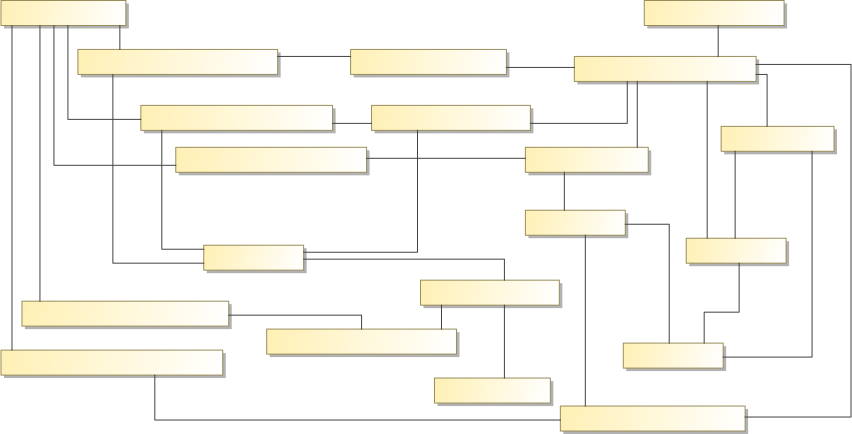
\includegraphics[scale=0.45]{img/uc2_test_config}
 \caption{Object diagram showing the use case as mapped test}
\end{figure}
The function mappings are done in the current solution, by manually writing up the logic needed in a support library, that in many situations reuse the framework directly. For instance, for every service, we have made a client class that, similar to RMI or WSDL handles all the low-level serialization and deserialization work. 

This enables us, in our tests to merely require that an interface (a client of it, that is) is provided to use, rather than having to explicitly elaborate the code in the test case.

%TODO Brief discussion on randomizers.

\begin{figure}
 \centering
 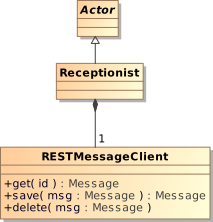
\includegraphics[scale=0.60]{img/support-tools-recepionist-example}
 \caption{support-tools-recepionist-example}
 \label{fig:support-tools-recepionist-example}
\end{figure}

%\begin{figure}
% \centering
%\missingfigure[figwidth=6cm]{This is some text that is with the todo and in the figure}
% \caption{support-tools-recepionist-example}
% \label{fig:support-tools-recepionist-example}
%\end{figure}

\begin{figure}[h]
%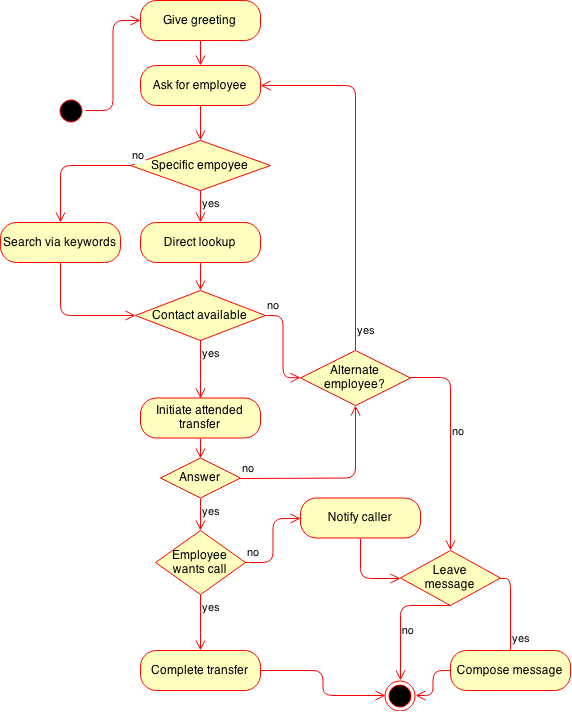
\includegraphics[scale=0.4]{img/activity_diagram_receptionist}
\centering
\caption{Activity diagram for the receptionist actor}
\label{fig:activity_diagram_receptionist}
\end{figure}


%\section{Related work}
%\subsection{Writing requirements as tests}
%\subsection{Writing requirements in formal language}

\section{Brainstorming}
Whenever there is a new use case, a change to an existing use case, or simply a definition, the system should try to generate tests from the new information. If this step fails it is likely due to insufficient concept mappings. From here, a software engineer must manually map individual definitions to system macro-functionality or, possibly the use case could be linked to an existing manually written test, if the generation step is not possible for some reason. A mockup of a user interface is shown in figure \ref{fig:use_case_editor_mockup}.

% Something about generating partially-automated tests, where the system sets up everything for the customer and then notifies them about the next steps they have to take to move the test forward.

\section{Extracting semantic}
Example; in the use case it is stated that a call is hung up and a callee awaits this event. The lifeline of the call is however not tracked and to be able to properly assert the true state of this, the code macro needs to into account this lifeline and reflect on which assertions hold for every stakeholder that has knowledge of the call. % TODO: Elaborate the example and explain that a phone call is a good example because it has an A and B-leg and potentially a system that tracks its state.

\subsection{Letting the customer inject semantics}

There are two basic approaches to letting the customer inject semantics into the requirements. The first is to do a full up-front declaration of every term used within the problem domain and supply this as a toolbox for the customer %todo example.
The other approach is to do it on the go by outlining concepts as stubs whenever they appear. This approach is similar to what is used in wiki software. %todo eaxmple

\section{Class-responsiblity-collaboration cards}
%Nouns should turn into the classes of the card, verbs typically turn into the responsibilities of the card, and collaborators are the other cards with which the card will be interacting with.
%FROM: http://en.wikipedia.org/wiki/Class-responsibility-collaboration_card

\subsection{Metrics}
% How many lines of code is the support tools? The middleware framework?
% How is it compared to the activity count in the activity diagram?

\section{Requirements as communication platform}

\section{Use case translation}
%\section{Object tracking} NOTE: Maybe something about object lifecycles (and statemachines for them) here.

\section{Test case state}
A test consists of three basic steps; setup, run and teardown. Setup and teardown is different from pre- and postcondition in that they are unrelated to the test itself, they merely make sure that objects are initialized with right values and, in general, are in the state that the test expects.

There needs to be an executable domain model programmed, not necessarily complete, but the concepts covered in the use cases should at least be there. So for \ref{fig:uc2}. We need at least a class representing the actor ``Receptionist'', and a class representing a message. The actions performed by the actor could then either be class methods, or simply functions taking the primary actor (or more exact; classes of the actor), as an argument.

\label{sec:test_case_state}

\section{Test case example}
\begin{lstlisting}
void use_case_1 (Receptionist receptionist) {

   MessageObjectFactory messageObjectFactory = new MessageObjectFactory();
   Message message = messageObjectFactory.create();

   // Preconditions
   Matcher.has (selected_contact (receptionist));

   // Use case body 
   receptionist.types_in(message);
   receptionist.sends(message);
   receptionist.marks_state_idle();

   // Postconditions 
   Matcher.is_true (is_stored (message));
   Matcher.is_true (is_idle (receptionist));
}
\end{lstlisting}

\begin{figure}
  \centering
 
  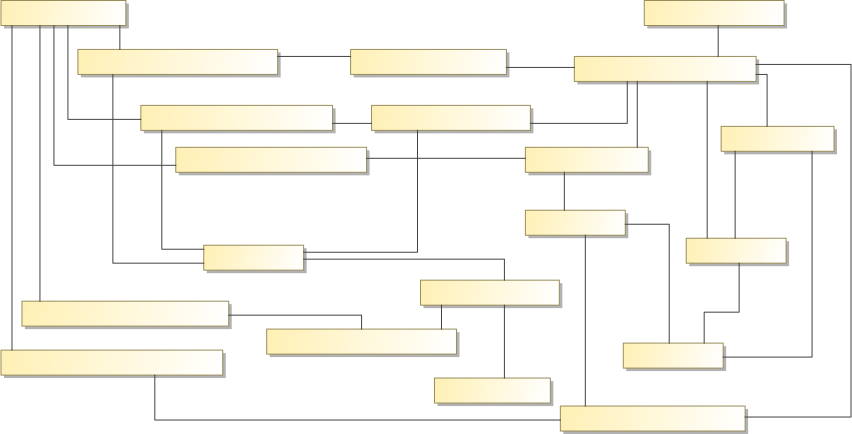
\includegraphics[scale=0.65]{img/uc2_test_config}
  \caption{object diagram depicting the configuration of use case 2}
  \label{fig:uc2_object_diagram}
\end{figure}

\section{Targeted requirements}
We've chosen to focus on the requirements that involves core features from the Receptionist actor point of view. These are, on a high level;
\begin{description}
  \item[Manage calls:] Being able to technically handle calls by performing receive, park, transfer and hangup action.
  \item[Process calls:] Being able to process calls in the context of a dialed reception. This involves having access to data about the reception and its contacts. Being able to dial them, or send them a message.
  \item[Manage message:] Being able to send out messages to contacts, view and resend existing messages.
\end{description}

\section{Structuring use cases}
In order to help the computer make more sense of our use cases, we need to define to it what a use case is. But since a use case is neither strictly defined nor standardized anywhere, we need to pick a suitable representation.
To help us extract some machine-understandable structure -- or merely semantics -- of use cases, we assume that we are working on ideal, well-formed use cases. This abstracts some of away the informal ambiguity, which is notoriously omnipresent in requirements, and will aid us when we try to derive what is needed from use cases in order to generate executable tests from them.\\\\
The first problem we need to solve is the level of use case writing, and template -- as there are many way of writing use cases. 
%TODO More discussion.
We have decided on using a fully-dressed use case template\cite{larman2005} as a guideline for the basic structure of the use case. In this, we have some key concepts that we need to address in our translation model. The main focus are concepts which provide useful information to generate tests from.

\section{Use case concepts}
This section discussed the individual components of a use case in the perspective of converting it into an executable test. But before venturing forth, we need to outline the concept of \emph{system state}, as it is referred in the following sections.

\subsection{System state}
Well-formed use cases  know are completely self-contained\cite{larman2005} in the way that every action and alternative, for a given actor, may be put into a single (large) use case. Use cases may also specify some expectations to the system state. This is what is defined as preconditions. If we, however, maintain the system state analogy, we can regard use case executions as mutation functions that affect the global system state.\\\\
A simple example; a actor \emph{accountant} has a use case \emph{accountant creates invoice}. This use case requires that the \emph{accountant} actor has previously been created. The creation could be provided by the \emph{admin} actor's \emph{admin creates accountant} use case.
\begin{figure}[h]
\includegraphics[scale=0.75]{\imgdir system-state-machine-relations}
\centering
\caption{State machine of perceived system state}
\label{fig:system-state-machine-relations}
\end{figure}
In summary, the \emph{accountant creates invoice} effectively has a precondition that is provided by \emph{admin creates accountant} to make the global state match what is expected to execute the \emph{accountant creates invoice}. The concept is illustrated in figure \ref{fig:system-state-machine-relations} where \emph{Use Case 1} is a prerequisite to \emph{Use Case 2}, but \emph{Use Case 3} has no prerequisites. In order to reach completion (termination) and coverage of \emph{Use Case 2}, \emph{Use Case 1} has to be executed.\\
Each use case state (an example is \textbf{UC1} in figure \ref{fig:system-state-machine-relations}) is a super-state that contains the state space of every alternative scenario. An example is shown in figure \ref{fig:system-sub-state-machine-relations}, where \\dots %TODO
\begin{figure}[h]
\centering
\caption{Example sub-states of a use case}
\label{fig:system-sub-state-machine-relations}
\end{figure}

\subsection{Primary actor}
The primary actor is important, as this is the stakeholder that defines the perspective and scope of the test. The primary is the person that starts the use case via an active action, or receives a start signal from another actor -- the system for instance. The primary actor should also -- as a minimum -- be part of the main scenario.

\subsection{Preconditions}

To achieve the minimum implementation, we cut away the optional precondition that may be covered by other use cases. After this, we see an implicitly \emph{ordered list of actions} that we need to succeed in order for the test to be a success. There is an actor that performs an action at each step. The system, in its entirety, may also be referred to as an actor as it is also capable of performing actions.


\section{Executable use case}
This section discusses a programming model and possible system designs that supports executing use cases. The basic concept is that every test is regarded as a function.
%Put this in; how many functions are in a test?

\subsection{Environment}
\textbf{!Unfinished!}\\
Executing the use case can be considered a long function call-chain. Each new function call passes along the current global state onto the next procedure. This method of passing along the state is a common pattern is interpreters and compilers, where the global state is referred to as "the environment". In our test-case compiler we adopt this approach. One of the large benefits is to have the ability to have an exit procedure that performs state clean upon exit of every use case. These procedures should run regardless of exceptions raised within the call-chain, but respond to them. This behavior is identical to the functionality seen in "teardown" functions in test framework for programming languages. See section \ref{sec:test_framework_programming} for a discussion on these frameworks.\\\\
The environment should contain the current state within the scope of test currently running. By state is meant any objects created or modified during the test.
The expression of a use case that consists of $n$ statements then becomes: 
\begin{equation}
Postcondition \rightarrow S_n \rightarrow S_{n-1} \rightarrow \dotsb \rightarrow S_2 \rightarrow S_1 \rightarrow Precondition \rightarrow env
\end{equation}
The expression function is applied to the statement, then the result is applied to the matcher which then returns a success or failure value depending on the outcome of the evaluation.
%\texttt{matcher expression} ($s$)

%\begin{algorithmic}
%\If {$i\geq maxval$}
%    \State $i\gets 0$
%\Else
%    \If {$i+k\leq maxval$}
%        \State $i\gets i+k$
%    \EndIf
%\EndIf
%\end{algorithmic}

\subsection{Mapping entries}
Any use case statement may be mapped to an assumption, an error or an assumption.

\subsection{Mapping branches}
Use cases may branch out and go to alternatives actions. These branches are associated with errors, and may be difficult to emulate. One possibility is to use an assumption mapping here, and treat the event or decision as having occurred. For active decisions taken by the primary actor, for example an action taken to better serve a customer request, it is easy to assume. Injecting errors in a running system is something else entirely... %TODO Finish.

\subsection{Determining paths}
%This is, most definitely a non-trivial problem.
In order to find all possible paths in a use case, the easiest way is to represent it as a graph and use a depth-first search or the more efficient one based upon Warshall's Theorem\cite{rubin1978enumerating} to emumerate them. Once a list of paths is retrieved, it is possible to convert every path, which is essentially a list of active actions either performed by, or affecting, the primary actor.\\\\
This list will be translated into a test by converting it into code snibblet, and join them together in a code block that becomes the body of a test function.

Back edges can occur, and this raised the bar, as it introduces loops.

%The basic rules for path collection is;

\subsection{Detecting logic errors in use cases}

\begin{description}
  \item[Skipping actions may be prohibited:] Should it be possible to jump ahead in the use case?
  \item[Primary actor must participate:] .
\end{description}




%TODO Integrate and finalize notes below.

% A use case returns a outputstate which is composed by an outputlog (log messages). A list of assumptions or an error. An error is for when an expectation failed, or a system error occured. Assumptions are for use case entries that are mapped to assumption statements.



%\section{Test framework}
% You need to write a test framework containing object pools, factory classes aso.
%\subsection{Exploiting injected semantics}
%How may we benefit from additional semantics? We can identify rubbish postconditions, such as predicates that involve objects that are either not modified in the statements, or simply never referenced.

%\section{Evaluating a use case}
%A use case can be modeled as a function taking in a starting environment and returning a boolean value, so $U \rightarrow env \rightarrow bool$


%Test case; when does it end? in our case, the message-sending archtecture is defined to be a work-queue where the dispatcher is decoupled from the message sending, which is merely an enqueuer. If the postcondition for our test case had been; "Message is received by contact", then the test-macro function becomes increasingly large.
%Test cases may further introduce dependencies, such as messageStore

%On the interface side, we decided that 2xx series HTTP codes where mapped to normal responses, and 4xx and 5xx to execeptions. 1xx and 3xx series are unused in our stak, and thus, unmapped. But it provides us with a good tool for -- on the client -- to explicitly state which replies should go where, and how they should be handled.


\subsection{Running the analysis}
Having a set of definitions, we can detect actors and concepts from textually analysing the text of every UseCaseEntry object. The analysis is quite simple, and merely looks for occurrences of the definition by comparing strings.

\subsection{Use case paths}
\begin{figure}[!htbp]
\centering
\begin{tikzpicture}[->,>=stealth',shorten >=0.8pt,auto,node distance=1.8cm,
thick,
visited node/.style={circle,fill=blue!20,draw,font=\sffamily\bfseries},
extension1 node/.style={circle,fill=orange!20,draw,font=\sffamily\bfseries},
chosen node/.style={circle,fill=green!20,draw,font=\sffamily\bfseries}]

%Scenario
\node[chosen node] (s1) {$s_1$};
\node[chosen node] (s2) [below of=s1] {$s_2$};
\node[chosen node] (s3) [below of=s2] {$s_3$};
\node[chosen node] (s4) [below of=s3] {$s_4$};
\node[chosen node] (s5) [below of=s4] {$s_5$};

%Extension 1
\node[visited node] (e1_1) [left of=s2] {$e_{1.1}$};

%Extension 2
\node[extension1 node] (e2_1) [right of=s4] {$e_{2.1}$};


%Paths
\path[every node/.style={font=\sffamily\small}]
(s1)   edge node [] {} (s2)	
(s2)   edge node [] {} (s3)
       edge node [] {} (e1_1)
(s3)   edge node [] {} (s4)
(s4)   edge node [] {} (s5)
       edge node [] {} (e2_1)
(e1_1) edge[bend right] node [] {} (s3)
(e2_1) edge[bend right] node [] {} (s2)
;
\end{tikzpicture}
\caption{Graph depicting different paths through a use case}
\label{fig:application graphs}
\end{figure}


%TODO add something about detection of loops.
Extensions may be covered in two ways. Just test the single extension with respect to the main scenario (the ``happy path''), or with respect to the other extensions as well.

\subsection{Capabilites of an actor}
If we were to add additional domain knowledge to the use cases, then we would also be able to extract capabilities easily.
%yada yada, use case example: actor does something to some other thing
% it means the the actor can do something to some other thing.

\subsection{Providing initial information}
%How to add receptions, users and other stuff?
%Could this be done with a use case as well?

\subsection{Configuration environment}
How do we define which objects are currently in the test harness? In our implementation, we have made a configuration file that, potentially could be auto-generated from a description of which domain types the objects have, what their internal data is, and when they need to be present.